\documentclass[a4paper,10pt]{article}
\usepackage[utf8]{inputenc}
\usepackage{amsmath}
\usepackage{graphicx}
\usepackage{float}
\usepackage{xcolor}

\usepackage[tmargin=1.0in,bmargin=1.0in, lmargin=1.25in, rmargin=1.25in]{geometry}


%opening
\title{Readme}
\author{Thomas Bellotti}

\begin{document}

\maketitle

\tableofcontents

\section{Brief description of the most important classes}
Since the whole project uses templates, almost all the classes are implemented in .h files stored in the folder \texttt{include}.
We now provide a brief description of what the most important classes do.
\subsection{Cell}
This class implements the notion of cell in a quadtree. Normally, the user does not have to directly use or interact with this class, which is the base brick of the class QuadTree and Pixel which will be introduced further.
\subsection{QuadTree}
This class implements the concepts of quadtree mesh, containing a smart pointer to a Cell, which is top of the tree.
The foundamental calls which a user should be aware of are:
\begin{itemize}
 \item The constructor, of course.
 \item \texttt{void buildUniform(const unsigned char)}, which constructs a uniform mesh with level specified by its argument.
 \item \texttt{void updateWithLevelSet(const LipschitzFunction<T> \&)}, which updates the mesh according to a criterion based on a level-set function (see presentation).
 \item \texttt{void updateQuadTree(const RefinementCriterion<T> \&)}, which does the same according to an arbitrary criterion given as argument.
 \item \texttt{void exportMeshTikz(const std::string \&, bool) const}, which lets us to export a \LaTeX file with a TiKz figure inside which allows us to plot the mesh we have constructed. 
 \item \texttt{T simpleIntegration(const std::function<T(Point<T>)> \&) const}, which performs a ``naive'' (see presentation) integration of a function (\texttt{T} is the template parameter).
 \item \texttt{T thirdOrderGaussianIntegration(const std::function<T(Point<T>)> \&) const}, does the same using a third order Gaussian quadrature rule.
\end{itemize}

\subsection{Pixel}
This class inherits from Cell and adds just an RGB value on each cell. It implements the notion of ``generalized'' pixel of an image.

\subsection{Image}
Though our concept of image is represented by a quadtree, this class does not inherit from QuadTree since most of the features we introduce are not exactly the same and we prefered to keep them separated.
The most important functions of this class from the user's point of view are:
\begin{itemize}
 \item \texttt{void createFromFile(const std::string \&)}, which given a file in PPM format (we wanted to avoid to use external libraries for the sake of simplicity), parses and stores the corresponding image in our data structure.
 \item \texttt{void simplifyImage(double)}, given a threshold as argument, is compresses (simplifies) the image based on the color variance (see presentation). Typical values of the threshold are between $0.01$ (high quality, low compression rate) and $0.05$ (very low quality, high compression rate).
 \item \texttt{void saveImage(const std::string \&) const}, saving the image, as for the quadtree, in \LaTeX~format.
\end{itemize}

\subsection{RefinementCriterion}
This is a small yet important class of the project. It is an abstract class containing the following \texttt{virtual bool operator()(std::shared\textunderscore ptr<Cell<T>> arg) const} which should tell the system if the cell pointed by the argument should be refined (split) or not.

Custom criteria (some of which are already implemented) must inherit from this class and override the method we have just presented.


\section{Compile the project}
In order to \textbf{compile} the whole project, simply use:
\begin{center}
 \begin{verbatim}
  make
 \end{verbatim}
\end{center}
in the project folder. Notice that we have slightly changed the flags, using \texttt{C++14} instead of \texttt{C++11} in order to slightly use its features and no flag is applied to the compilation of the \texttt{MPI} sources since it would stop compilation due to errors, which are not generated by our source code, but rather by the way the \texttt{MPI} distribution has been compiled.
As usual, one can use
\begin{center}
 \begin{verbatim}
  make distclean
 \end{verbatim}
\end{center}
to clean the whole project.

\section{Examples and binaries}
Rather than a ready-to-use application, we provide a lot of examples and test which use all (or almost) the features of our classes.
We describe them in this section.

\subsection{Ready-to-use binaries}
\begin{itemize}
 \item \textbf{bin/imagecompression}. This is implemented in \texttt{src/main/imagecompression.cpp} and should be called with three arguments: the name of the input file (in .ppm format), the name of the output file (which will be a \LaTeX file) and the threshold for the image compression.
 
 It performs the compression of the image according to our method. Notice that the image must be square, with number of pixels per side which is a power of $2$, for the sake of simplicity.
\end{itemize}

\subsection{Ready-to-use functions}\label{foo1}
\begin{itemize}
 \item \textbf{src/parallel\textunderscore integration.cpp}, which is compiled to give \texttt{build/parallel\textunderscore integration.o}, which contains the parallel function:
 \begin{center}
  \begin{verbatim}
double parallel_integration(const std::function<double(Point<double>)> & func, 
    unsigned order, const Point<double> & l_left, const Point<double> & u_right, 
    unsigned char min_lev, unsigned char max_lev, 
    const RefinementCriterion<double> & criterion)   
  \end{verbatim}
 \end{center}
This functions integrates the function \texttt{func} with the naive formula (\texttt{order} = 0) or the 3rd order Gaussian formula (\texttt{order} = 1) on a square domain of lower left corner \texttt{l\textunderscore left} and upper right corner  \texttt{u\textunderscore right} on a mesh of minimum level and maximum level given by \texttt{min\textunderscore lev} and \texttt{max\textunderscore lev}, which is refined according to \texttt{criterion}.

Notice that there are many requirements on the number of cores used and the minimum size of the mesh which are explained inside the code, so have a look at it for further information.
\end{itemize}

\subsection{Example binaries}
\textcolor{red}{\textbf{Caveat}: In many examples, since inside the .cpp file we use absolute paths to provide ouput files, one may need to change them according to its distribution of the project in order to test the code. We do apologize.}
\subsubsection{General}
\begin{itemize}
 \item \textbf{bin/basic\textunderscore bricks}, compiled starting from \texttt{src/test/basic\textunderscore bricks.cpp}, which tests some of the basic calls which make the code working. It is not really interesting, it has been used mainly for debugging purpose.
 \end{itemize}
 \subsubsection{Quadtree meshes}
 \begin{itemize}
 \item \textbf{bin/test/quadtree\textunderscore highly\textunderscore adaptive\textunderscore mesh}, which has been compiled starting from the source code \texttt{src/test/quadtree\textunderscore highly\textunderscore adaptive\textunderscore mesh.cpp}. It tests the mesh adaptation with different criteria, outputing the figures in folders which can be specified in the source code (it needs to be adapted if the user changes path, which is likely to happen).
 \begin{figure}[H]
\begin{center}
\includegraphics[width=0.4\textwidth]{./figures/readme/level_set.pdf}
\end{center}
\end{figure}
This figure shows an example of output (once compiled with \LaTeX), but many more are possible.
\item \textbf{bin/test/quadtree\textunderscore time\textunderscore evolving\textunderscore mesh}, which tests the possibility of making a mesh evolving with time in order to implement selective refinement for time-dependent problems. It is compiled starting from the source code \texttt{src/test/quadtree\textunderscore time\textunderscore evolving\textunderscore mesh.cpp}
The logic is almost the same than in the previous test.
 \begin{figure}[H]
\begin{center}
\includegraphics[width=0.3\textwidth]{./figures/readme/frame0}
\includegraphics[width=0.3\textwidth]{./figures/readme/frame9}
\includegraphics[width=0.3\textwidth]{./figures/readme/frame15}
\end{center}
\end{figure}
\item \textbf{bin/test/quadtree\textunderscore other\textunderscore meshes}, which tests the mesh refinement using fancy criteria, also in order to build a fractal structure such as the Mandelbrot set.
 \begin{figure}[H]
\begin{center}
\includegraphics[width=0.95\textwidth]{./figures/readme/fractal}
\end{center}
\end{figure}
The source file is located at \texttt{src/test/quadtree\textunderscore other\textunderscore meshes.cpp}.
\item \textbf{bin/test/quadtree\textunderscore integration}, which tests the integration functions in QuadTree (without parallelism). It is implemented in \texttt{src/test/quadtree\textunderscore integration.cpp} 
\end{itemize}
\subsubsection{Parallel integration on quadtree meshes}
These are nothing but different tests for the parallel integration function presented in Section \ref{foo1}. They are also shown in the presentation, so we present them rapidly:
\begin{itemize}
 \item \textbf{bin/test/mpi\textunderscore pi}, implemented in \texttt{src/test/mpi\textunderscore pi.cpp}
  \item \textbf{bin/test/mpi\textunderscore gauss}, implemented in \texttt{src/test/mpi\textunderscore gauss.cpp}
   \item \textbf{bin/test/mpi\textunderscore square}, implemented in \texttt{src/test/mpi\textunderscore square.cpp}
    \item \textbf{bin/test/mpi\textunderscore unif}, implemented in \texttt{src/test/mpi\textunderscore unif.cpp}
\end{itemize}
They all take the following arguments: minimum level and maximum level, type of quadrature rule (0 for naive and 1 for Gaussian) and the type of mesh we use for the test (1,2 or 3), see inside the source or in the presentation for more on it.
Notice that the bash script \texttt{batch\textunderscore mpi\textunderscore test.sh} in the root of the project executes them in batch varying all the parameters and the number of cores.
\subsubsection{Image compression}
\begin{itemize}
 \item \textbf{bin/test/image\textunderscore compression}, which is compiled from \texttt{src/test/image\textunderscore compression.cpp}.
 It tests the compression of some sample images (contained in \texttt{media/images} for different threshold values. Notice that the output folder may need to be changed.
  \begin{figure}[H]
\begin{center}
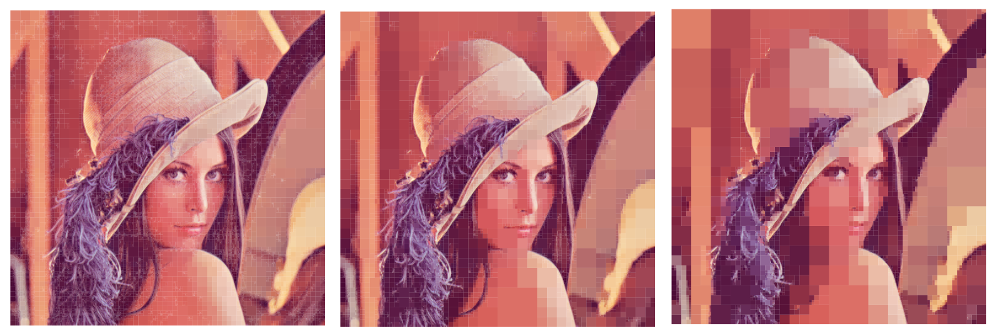
\includegraphics[width=0.95\textwidth]{./figures/readme/s4_comp_small}
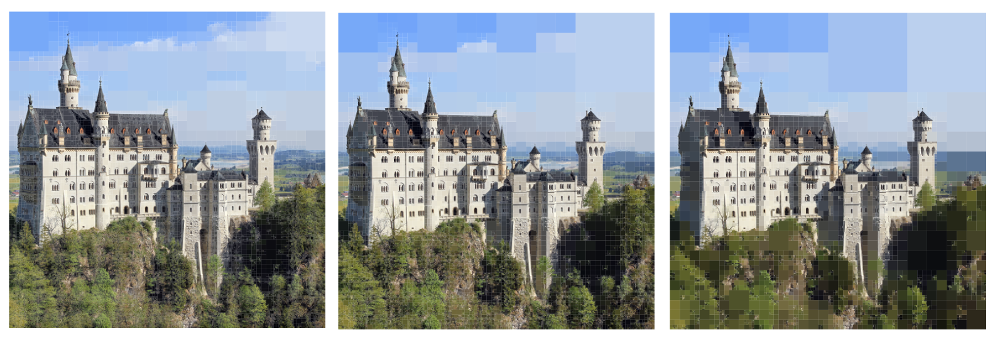
\includegraphics[width=0.95\textwidth]{./figures/readme/s2_comp_small}
\end{center}
\end{figure}
These are some of the examples of image compression.
\end{itemize}



\section{How to compile output images}
In order to compile the \LaTeX ~ files which are the output used to visualize the quadtree structures, both as meshed and images, one must have a complete \LaTeX ~ distribution of this system with the TiKz package installed.

For small figures, writing
\begin{center}
 \begin{verbatim}
  pdflatex file_name.tex
 \end{verbatim}
\end{center}
is sufficient. Nevertheless, if the figure is really complex, this could saturate the buffer of \texttt{pdflatex}. The easiest way of fixing this issue is to use \texttt{lualatex} instead:
\begin{center}
 \begin{verbatim}
  lualatex file_name.tex
 \end{verbatim}
\end{center}
which is slightly slower but allows to represent large images or meshes.

\end{document}
